\documentclass{article}

% Any additional packages needed should be included after jmlr2e.
% Note that jmlr2e.sty includes epsfig, amssymb, natbib and graphicx,
% and defines many common macros, such as 'proof' and 'example'.
%
% It also sets the bibliographystyle to plainnat; for more information on
% natbib citation styles, see the natbib documentation, a copy of which
% is archived at http://www.jmlr.org/format/natbib.pdf
\usepackage{jmlr2e}
\usepackage{geometry}
\geometry{verbose,a4paper,tmargin=20mm,bmargin=20mm,lmargin=10mm,rmargin=15mm}
\newcommand{\dataset}{{\cal D}}
\newcommand{\fracpartial}[2]{\frac{\partial #1}{\partial  #2}}
\setlength{\parindent}{0pt}

% For quoting
\usepackage{dirtytalk}
\usepackage{caption}
\captionsetup[figure]{font=footnotesize}
% For enumerations
\usepackage{enumerate}
\usepackage{bm} % bold math symbols (vectors)

% For manageable columns
\usepackage{multicol}
\setlength\columnsep{18pt} 

% For strikethroughs
\usepackage{soul}

\usepackage{xcolor}
\definecolor{red}{rgb}{1,0,0}
% To format the section titles nicely (not yet perfect)
\usepackage{titlesec}
\titleformat{\section}{\huge\sffamily}
\titleformat{\subsection}{\huge\sffamily}
\titlespacing{\section}{0pt}{\parskip}{-\parskip}
\titlespacing{\subsection}{0pt}{\parskip}{-\parskip}
\titlespacing{\subsubsection}{0pt}{\parskip}{-\parskip}

% For distance between figures/tables and their caption
\usepackage[font=small,skip=2pt]{caption}
\captionsetup[table]{font=small,skip=4pt}

% For distance between caption of figure/table and normal text
\usepackage{etoolbox}
\BeforeBeginEnvironment{figure}{\vskip-1ex}
\AfterEndEnvironment{figure}{\vskip1ex}
\BeforeBeginEnvironment{table}{\vskip-1ex}
\AfterEndEnvironment{table}{\vskip-4ex}


% Graphics package
\usepackage{graphicx}
% For nice plots??
\usepackage{pgfplots}
% For making hyperlinks dark blue
\usepackage{color}
\definecolor{myblue}{rgb}{0 0 0.4}
\definecolor{grayishgray}{rgb}{0.5, 0.5, 0.5}

%Math
\usepackage{mathtools}
\usepackage{amsmath}
\DeclareMathOperator*{\argmax}{arg\,max}
\usepackage{amsfonts}
\usepackage{amssymb}
\usepackage{algorithm}
\usepackage{algpseudocode}
\usepackage{caption}
\usepackage{subcaption}

% To allow interactive clicking on references 
\usepackage{hyperref}
\usepackage{nameref}
\hypersetup{
    colorlinks,
    citecolor=myblue,
    filecolor=myblue,
    linkcolor=myblue,
    urlcolor=myblue
}

\usepackage{comment}
% Heading arguments are {volume}{year}{pages}{submitted}{published}{author-full-names}

% Short headings should be running head and authors last names

\ShortHeadings{Gruber, Vogelsang, Born - TNM Final Project Report }{}


% Solving reference frames based on spatial similarity
\firstpageno{1}

\usepackage{nccmath}
\addtolength{\footnotesep}{2mm}

\begin{document}
\title{The Influence of Stimulus Nature on Probabilistic Inference in Generative Models of Behavior and its Physiological Correlates}

%Influence of stimulus nature and skin conductance response signals on the $\omega_2$ parameter of a Hierarchical Gaussian Filter and its temporal re-interpretation


%Influence of stimulus nature and peripheral physiological signals on a generative model of behavior and its parametric reinterpretation as a temporal window of integration - Alternative? 

\author{\name Moritz Gruber\textsuperscript{1}, Lukas Vogelsang\textsuperscript{1}, Jannis Born\textsuperscript{1}}
\maketitle

\vspace{-1cm}
\indent \textbf{1} \textit{Institute of Neuroinformatics, ETH Z\"urich and University of Z\"urich, Switzerland}  \\ \\
\bigskip

\begin{abstract}
The current state of psychiatric diagnostics calls for a transition from phenomenology to aetiology and from subjective to objective, physiologically interpretable classification criteria. 
%In computational psychiatry, such measures of internal states are made accessible by means of generative models, where both physiology and behavior can be mathematically described in a bottom-up manner.
%Within this broader context, the study described herein aims first at devising a quantitative, potentially disease-relevant measure of behavioral states by modeling how aversive versus neutral stimuli bias behavior in an audio-visual learning task. 
% Maybe zusammenfassen als - J
Within the context of computational psychiatry non-invasively shedding light onto internal states by means of generative models, the presented study aims at devising a quantitative, potentially disease-relevant measure of behavioral states by modeling how aversive versus neutral stimuli bias behavior in an audio-visual learning task. 
In addition, we investigated possible peripheral physiological correlates of computational quantities delivered by the Hierarchical Gaussian Filter (HGF). Finally, we sketch a temporal perspective on $\omega_2$, a key parameter in the HGF, and compare hierarchical Bayesian and non-hierarchical non-Bayesian models of learning (HGF and Rescorla-Wagner). In our experiment, behavioral data and skin conductance measurements from $n = 16$ subjects were acquired. Our findings suggest a bidirectional effect of aversive stimuli on behavior in two different subgroups and a promising hint at the existence of canonical physiological responses to prediction errors pertaining to %both polarities.
the early levels of the generative hierarchy. % J
%We conclude with a theoretical perspective on $\omega_2$, relating it to  hierarchical Bayesian (HGF) and non-hierarchical, non-Bayesian models (Rescorla-Wagner) of learning. 
Overall, our results, if replicated on a more significant --- perhaps clinical --- sample, represent a modest step towards the sorely needed, mechanistic psychiatric diagnostics by bridging the gap between adherents to the Bayesian brain hypothesis and adjacent neuroscientific fields.
\end{abstract}

\vspace{2mm}
All the code is available on \href{https://github.com/tnm-finalproject/TNM_project}{https://github.com/tnm-finalproject}. \\
\vspace{2mm}

\textsf{\textbf{KEYWORDS}: computational psychiatry, generative model, hierarchical gaussian filter, galvanic skin response, skin conductance response, prediction error, Bayesian brain, temporal window of integration, Bayesian model selection}
\begin{multicols}{2}
\section*{Introduction}
\label{sec:intro}
\subsection*{Towards an objective and quantitative strategy for diagnostics in psychiatry}	
\textit{The status quo.} Traditionally, psychiatric diagnostics are performed on the basis of a classification dictated by the Diagnostic and Statistical Manual (DSM), or similar, which comprises a comprehensive list of psychiatric disorders along with the signs and symptoms that make patients eligible for diagnosis. In the case of schizophrenia, one of the most prevalent psychiatric disorders \citep{Saha2005}, this list includes delusions, hallucinations, anhedonia, flat affect, asociality, disorganized behavior, and many more. According to the DSM, exhibiting at least two symptoms (at least one of the positive variety) over the course of at least one month is sufficient to obtain the label \say{schizophrenic}. While this approach to diagnostics has proven effective in dealing with great numbers of returning soldiers post Wold War II, it inherently suffers from at least two major flaws. First, due to the diverse array of possible genetic predispositions and environmental risk factors, the pool of patients under the same diagnostic umbrella inevitably becomes highly heterogeneous in terms of pathologies. Secondly, there is no systematic and informed way of prescribing drugs, let alone predicting treatment courses: Drugs tend to be prescribed in a trial-and-error fashion, often based on what side effects the individual patient could tolerate best. \\ 
\textit{The computational approach.} Deeming this status quo untenable -- both for clinicians and patients, but also their relatives -- the emerging field of computational psychiatry has set out to develop methods that allow for the objective and quantitative classification of patients. Moving away from subjective reports of symptoms, towards diagnostics that are grounded in aetiology rather than phenomenology, requires external sources of information in the form of neuroimaging or behavioral data. Prima facie, one could imagine that differential diagnosis may be feasible based on raw, anatomical data, such as magnetic resonance imaging (MRI) scans. While projects of this kind have been successfully undertaken \citep{Liu2017}, they bring us no closer to the bottom-up understanding of disease mechanisms that would enable us to prescribe targeted treatments. \\
\subsection*{Generative models of neuroimaging data}
A more promising approach rests in the concept of \textsf{generative modeling}, in the context of which physiologically interpretable, computational models of the brain are constructed based on externally acquired data. More technically, those models mathematically describe the probabilistic links between hidden states of the brain and the noisy measurements we acquire using MRI or electroencephalography (EEG). The result of this approach is a set of subject-specific parameters that can be readily mapped onto physical entities (such as the average weight of excitatory long-range connections between two specific brain regions) and therefore exploited for a white-box classification into disease cohorts. The work of \cite{VanLeeuwen2011} on synaesthetes serves as illustrious proof of concept of this approach: Based on an anatomically informed set of prior models, two groups of different phenomenology, namely the \say{projectors} and the \say{associators}, could be reliably distinguished, which has led to an understanding at the mechanistic level in terms of effective brain connectivity. Several similar studies within the clinical realm suggest that this approach can, in principle, be applied to assay specific neurophysiological parameters (\textit{e.g.}, potassium channel \citep{Gilbert2016} or NMDA receptor activity \citep{Symmonds2018a}, marking a significant step towards objective, quantitative psychiatric diagnostics.
\subsection*{Generative models of behavior}
Within the context of a theoretical framework he coined as the \textsf{Free Energy Principle}, Karl Friston argues that given the objective of minimizing energy expenditure, the brain's optimal policy is to hold and constitutively update a generative model of its inner and outer milieu, in an effort to avoid costly \textsf{actions} on the world or on itself (by changing its anatomy). The ensuing generative modeling approach of behavior rests on the Bayesian Brain hypothesis \citep{Friston2012}, which postulates a \textit{hierarchical} generative model within the brain that is aimed at minimizing statistical \textit{surprise}. At any point in time, an organism's objective to minimize surprise is accomplished in case it had perfectly predicted a prospective sensory input.  The computational quantity describing the mismatch between a prediction and the actual sensory input has been postulated as \textbf{prediction error}(PE).

The \textsf{Hierarchical Gaussian Filter} (HGF) is the most established computational framework designed to mimic these requirements \citep{Mathys2014}. For the simple case of predicting a series of binary outcomes, the model would be structured as follows: At the lowest level, drawing from a Bernoulli distribution yields a binary outcome. To account for dynamic changes in the probability of the latter distribution, the second level represents it as a Gaussian random walk, the \textsf{tendency}, whose variance in turn depends on a random variable at the third level, termed the \textsf{volatility}. The parameters that govern the dependencies between different layers in the hierarchy can be fitted to individual subjects, given behavioral data from a suitable task. In addition to those parameters, individual model fits also yield interesting computational quantities for each trial, such as \textsf{precision-weighted prediction errors (pwPEs)}, which can then be correlated to brain activity using conventional general linear models for fMRI. Following such an approach within the context of an audio-visual learning paradigm, \cite{iglesias2013hierarchical} found neurophysiological correlates of prediction errors at different levels of the generative hierarchy in different regions of the brain, e.g., low level PEs in the midbrain. \\

\subsection*{Motivation for presented work}
\label{sec:Q}
This project is geared towards investigating the following questions:
\begin{enumerate}[A.]
\item Do computational quantities also have \textit{peripheral} physiological correlates?
\item Does stimulus nature bias behavior in a sensory-motor learning task?
%\item If the second holds true, can this be used as a diagnostic tool in computational psychiatry? - presentation version, J
\item Can we derive a temporal interpretation of behavioral parameters that may serve as a  diagnostic tool in computational psychiatry?
% I'd like to emphasize the translational, bridging aspect here, aber ich fürchte dass das der TNU in den falschen hals fallen könnte. 

\end{enumerate}
Based on \cite{iglesias2013hierarchical}, we acquired behavioral data from 16 subjects in an audio-visual learning paradigm. Subjects were presented with a binary visual cue and subsequently asked to predict whether there will be an auditory stimulus or not. The difficulty of the task lies in the fact that the probabilities that govern the cue-stimulus contingencies change over time. In addition to behavioral data, we measured the participants' galvanic skin response over the course of the experiment. The details of the experimental setup are described in the \hyperref[sec:meth]{next section}.
\\ In the following, we will sequentially motivate each of these questions and elaborate on how our experiment serves to address them. \\
\vspace{1mm}

\textbf{A. Do computational quantities also have peripheral physiological correlates?}
%\subsection{Peripheral correlates of computational quantities?}
It is intuitively sensible that surprise, in the colloquial sense, draws attention by creating arousal. For instance, when absent-mindedly attempting to cross a street, and noticing a car frantically breaking, you become aware of the danger \textit{as a result of} an innate emotional response, triggered by the fact that your brain had not predicted this specific, highly salient input. Physiological responses such as increased heart rate, tense muscles and active sweat glands quickly ensue as a result of this near-fatal prediction error. Thus, it stands to reason that prediction errors--- even those of the milder variety--- or other abstract computational quantities, could in principle be assayed by reading out those peripheral states. Numerous studies have examined correlates of prediction errors on a variety of spatial scales ranging from the level of single-cell-recordings \citep{o2013risk} to widespread areas including millions of neurons \citep{brydevall2018neural}. Prior work extends from cognitive to behavioral manifestations of different subtypes of prediction errors \citep{iglesias2017models,den2012prediction}. However, only a handful of studies have attempted to unravel possible relations between the Galvanic Skin Response (GSR, or skin conductance) and a PE signal \citep{bach2010dynamic,spoormaker2011neural}. Since the polarity of skin conductance prediction error signals to unconditioned stimuli has been controversially discussed \citep{spoormaker2012additional}, we prefer using \textit{surprise} (rather than error) as a directionally agnostic term. Hence, we present an effort to deepen the understanding of the role of skin conductance as a potential correlate of prediction errors. In a nutshell, a GSR device acquires a time series of skin conductances which vary as a function of autonomic modulation of perspiratory gland activity. It had therefore long been deemed to be one of the most robust markers of emotional arousal and surprise.\\% vast implications if SCR would contain PE signal. 
The reason we judge the first question as having substantial value is that unraveling GSR as a resilient byproduct of specific types of prediction errors would carry implications for the ethos of the Bayesian brain hypothesis as follows. 
Let us reformulate the first question to: Is it possible to infer the belief about the occurrence of a binary event in the \textit{absence of a proper behavioral response}? Assuming the stereotyped response for situations \textit{with} a prediction error is orthogonal to the stereotyped response \textit{without} a prediction error, a GSR device could in principle be used to trace back the belief about the occurrence of the binary event. In a behavioral paradigm that involves tracking of the predictive power of a cue about the occurrence of such an event, following that approach for every trial yields a binary trace of event predictions. The inferred belief trace is structurally identical to the online recorded behavioral response trace (e.g. collected via keyboard) and as such, amenable to all analyses performed on the behavioral trace (e.g. by generative models of behavior like the HGF) and, more particularly, for a qualitative comparison of the respectively inferred model parameters. Given this hypothesis is correct, a practical application could be present in case a motorically highly demanding procedure is used to acquire the behavioral responses (or in case a patient suffers from tremor, e.g. like in Parkinson's disease). In that scenario, the skin conductance response (SCR) inferred response trace could more closely reflect the participant's actual belief than the noise-distorted behavioral trace. \vspace{2mm}
%The mere application of SCR as part of lie detection devices [QUOTE] raises expectations that it can access beliefs the participant could hide otherwise.
% MO: Hab gehört das sei mittlerweile umstritten, also sollten wir da vorsichtig sein. 
% J: Okay lieber raus, ist eh n unwichtiger fun fact

\textbf{B. Does stimulus nature bias behavior in a sensory-motor learning task?}
%\subsection{Do aversive vs. neutral stimuli bias behavior?}
Our experiment was designed to address a second question. 
In the first session of 150 trials, the auditory stimulus whose occurrence the participants were tasked to predict was a neutral, 200 Hz pure tone with a windowed onset. In the second session however, the tone was an aversive, sudden-onset white noise stimulus, at an amplitude calibrated to 90 \% of the individual acoustic pain threshold. Comparing HGF parameter fits between neutral and aversive sessions would hopefully shed some light onto how the nature of the stimulus confounds behavior. One hypothesis is that participants whose $\omega_{2}$, an additive term affecting the variance of the tendency (see \textsf{Methods}), increases in the aversive condition are more prone to erratic behavior, and vice versa. To investigate this hypothesis, subjects were asked to answer a short questionnaire where one of the questions was to rate how prone to anxiety and nervousness they judge themselves to be. \vspace{2mm} 

\textbf{C. Can we derive a temporal interpretation of behavioral parameters that may serve as a  diagnostic tool in computational psychiatry?}
%\subsection{Towards cognitively interpretable behavioral parameters as diagnostic tools}
We developed a complementary Pseudo-Bayesian framework to render the HGF differences in $\omega_{2}$-differentials between our participants intuitively accessible in the time domain. Specifically, we show that, under certain constraints, $\omega_{2}$ can be cast in terms of a \textsf{temporal window of integration} -- a measure that may represent one dimension in the multidimensional continuum that the field of psychiatry is spanning; a measure that is interpretable by people both inside and outside of the Bayesian community. 

%\end{multicols}
\section*{Methods}
\label{sec:meth}
\subsection*{Experimental Design}

The behavioral experiment was based on \cite{iglesias2013hierarchical} and consisted of two sessions \`{a} 150 trials each. The setup of one trial is displayed in \autoref{fig:exp}. Cues and cue-stimulus contingencies were governed by the following probabilities: 

\begin{ceqn}
\begin{align}
 p(\text{tone}|\text{square}) = 1-p(\text{no tone}|\text{square}) \\
= 1-p(\text{tone}|\text{circle}) = p(\text{no tone}|\text{circle}) \nonumber 
\end{align}
\begin{align}
p(\text{square}) = p(\text{circle})
\end{align}
\end{ceqn}

Every 30 trials, $p(\text{tone}|\text{square} )$ changed in a discrete fashion in the following order: 0.9, 0.1, 0.5, 0.7, 0.3, adding up to a total of 5 blocks \`{a} 30 trials each. Importantly, the two sessions differed solely in the nature of the auditory stimulus: a neutral, windowed onset 200 Hz tone in the first session and an aversive, sudden-onset white noise tone in the second session. \\

\begin{figure}[H]
\centering
\includegraphics[width=.48\textwidth]{exp.png}
  \caption{ Each trial was compounded by a binary visual cue shown for 400 ms, followed by a 1200 ms response time, a 1000 ms auditory stimulus presentation and a variable inter-trial-interval of 1000 ms $\pm$ 500 ms.}
  \label{fig:exp}
\end{figure}%

\subsection*{Construction of Galvanic Skin Response device}

In electrical terms, the skin can be modeled as a series of parallel resistors whose conductivity (or inverse resistance) increases with secretion of sweat. Because resistances are hard to measure using a microcontroller, the measuring device is based on a voltage divider, where R1 is a fixed resistor and R2 represents the skin. Custom-built electrodes were fabricated from 5-Rappen coins, which were selected because of their ratio of highly conductive copper (92 \%). An \texttt{\href{https://www.arduino.cc}{Arduino Uno}} microcontroller was connected to the voltage divider, supplying 5 Volts to R2 and the node between R1 and R2 was connected to a 10-bit analog-to-digital converter (ADC) (see \autoref{fig:gsr-setup}). Thus, the measured values range from 1023 (short circuit) to 0 (open circuit). To balance the trade off between sensitivity and dynamic range, we selected R1 for each individual subject such that the baseline input value was in the vicinity of 600. Typically, resistors between 100 k$\Omega$ and 1 M$\Omega$ were used. 
The \texttt{Arduino Uno} was programmed to interface with \texttt{MATLAB}, providing samples at a rate of about 65 Hz. 


\vspace{2mm}
\subsection*{Analysis of Galvanic Skin Response data}
The measurements were acquired with the aforementioned microcontroller at a sampling rate that varied between 60 and 70 Hz. Prior to analysis, time stamps of the GSR signals were synchronized with the time stamps from the behavioral measurements. Next, data was downsampled to equidistant samples every 20 milliseconds (50 Hz) using \texttt{MATLAB}'s nearest neighbor interpolation (\texttt{interpn}). The \texttt{Arduino} backend limited the range of returned conductances to a 10-bit representation thus obliterating interpretation of the absolute values of the signal. For the following steps, \texttt{Ledalab}, an established \texttt{MATLAB}-based toolbox for analysis of GSR data was used \citep{karenbach2005ledalab}. By means of a continuous decomposition analysis, the phasic component of the GSR signal (to which we refer as skin conductance response, SCR) was extracted \citep{benedek2010continuous}. The tonic component (skin conductance level) instead, was excluded from post-hoc analysis as it fluctuates in the range of seconds to minutes rather than 1-5 seconds post-stimulus as the SCR. \\
\begin{figure}[H]
\centering
\includegraphics[width=.48\textwidth]{arduino.png}
  \caption{Circuit diagram of  the GSR measuring device based on an Arduino microcontroller and 5-Rappen coins as electrodes. The voltage divider referenced in the text consists of R1, the fixed resistor and R2 (not annotated), which pertains to the combined resistance of electrodes and skin.}
  \label{fig:gsr-setup}
\end{figure}%


\subsection*{Experimental Procedure}

\textit{Initialization}. First, subjects were handed an individual sheet containing instructions (see GitHub repository) and a brief questionnaire, which they were instructed to start filling out. To guarantee their anonymity with respect to data analysis, subjects were first asked to pick an ID from an envelope and write it on their sheet. Next, any remaining questions as to the experimental procedure were answered, ensuring that no participant was told how or when the predictive strengths of the cues would change. Finally, to improve motivation, subjects were told that they would receive a performance-dependent compensation of 4 Rappen per correct trial, i.e., a maximum of 12 CHF. \\
\textit{GSR recording}. Electrolyte gel was applied to two spots on the participants’ left hand and custom-made GSR electrodes were thoroughly mounted using medical tape. The data was recorded using a custom-written \texttt{MATLAB} interface specifically designed to sample GSR data at an effective sampling frequency of around 65 Hz. \\ 
\textit{Stimulus amplitude calibration}. Before starting the experiment, the amplitude of the aversive stimulus was calibrated for each participant individually to maximize comparability. To this end, subjects were fitted with over-ear headphones, presented with a randomized sequence of the aversive white noise stimulus of 1000 ms duration at different amplitudes and were asked to rate each one on a painfulness scale from 0 (harmless) to 100 (pain threshold). Subsequently, the stimulus amplitude corresponding to 90 \% of their individual pain threshold was extrapolated, presented to the participant for approval, and adjusted if necessary.\\
\textit{Experiment}. Subjects sat in front of a screen with their left hand laying on the table (and being recorded from) and their right middle and index fingers on a keyboard to provide behavioral output. Presentations of cues and stimuli as well as recordings of behavioral and physiological data were carried out in \texttt{MATLAB}.\\

\subsection*{Questionnaire}
During and after the experiment, subjects were asked to fill out a questionnaire (available on \href{https://github.com/tnm-finalproject/TNM_project/blob/master/instruction_sheet.pdf}{GitHub}) consisting of three questions to be answered on a scale from 0 to 10. 
\begin{enumerate}
\item How do you feel today?
\item In general, how easily do you become nervous or anxious in everyday life?
\item How well do you believe you performed the task?
\end{enumerate}
A priori, the first question was designed to potentially eliminate significantly underperforming subjects with greater confidence, while the other questions would be plotted against experimental data and differences in model parameters (see \textsf{Results}).  \\

\subsection*{Assessment of Performance Profile}
\label{sec:ass}
For a first assessment of performance profiles, we analyzed subjects' responses in the five 30-trials blocks that are governed by different cue-stimulus-contingency probability distributions. This analysis was carried out for the neutral and aversive condition separately. A subject's condition-wise performance score is defined as the proportion of correct responses. A correct response is defined with respect to the underlying conditional probability distribution: in a block where cue-stimulus-contingency 1 will occur with a probability greater than 0.5, the correct response will be cue-stimulus-contingency 1; otherwise it will be 0. As such, the correct response is independent of the feedback received in any particular trial. Responses from the third block were disregarded for performance analysis as the conditional probability was at chance level. \\
% This is in accordance with the procedure described in \citep{iglesias2013hierarchical}. - Ist das so? J \\


\subsection*{Data Purge}
\label{sec:purge}
The experiment was conducted with a cohort of $N=16$ subjects. Due to high trial failure rates (i.e. no valid prediction inserted in $>10\%$ of the trials), 4 subjects were discarded from all analyses. In addition, several hardware problems in the GSR measuring device, in particular (1) high-frequency noise induced by concurrent charging and sampling, (2) long-range drifts caused by metal keyboards disturbing the electric circuit and (3) a lack of conductive paste (as used for EEG), forced us to purge all but the last 4 GSR recordings we had gathered. \\

\subsection*{Model-based Analysis: Hierarchical Gaussian Filters} 
\label{hgf-methods}
\subsubsection*{Theory}
In the context of the HGF \citep{Mathys2014}, a binary outcome can be \textit{generated} by sampling from a Bernoulli distribution (\ref{eq:bern}), whose parameter is a sigmoid of the \textsf{tendency} $\mathbf{x_{2}}$ (\ref{eq:x2}), which evolves as a Gaussian random walk over time ($k$). The variance of the tendency depends on the third level of the hierarchy, the \textsf{volatility} $\mathbf{x_{3}}$, in an exponential parameterized by a multiplicative parameter $\kappa_{2}$ as well as an additive parameter $\omega_{2}$. The volatility is also described by a Gaussian random walk with fixed parameter $\omega_{3}$.

\begin{align}
&\rm p\big(\mathbf{x_{3}^{(k)}}|\mathbf{x_{3}}^{(k-1)}\big) = \mathcal{N}\big(\mathbf{x_{3}}^{(k-1)},\omega_{3}\big) \\[1em]
&\rm p\big(\mathbf{x_{2}^{(k)}}|\mathbf{x_{2}}^{(k-1)},\mathbf{x_{3}}^{(k)}\big) = \mathcal{N}\big(\mathbf{x_{2}}^{(k-1)},\rm exp(\kappa_{2}\mathbf{x_{3}}^{(k)}+\omega_{2})\big) \label{eq:x2}\\[1em] 
&\rm p\big(\mathbf{x_{1}^{(k)}}|\mathbf{x_{2}^{(k)}}\big) = \rm Bernoulli\big(s(\mathbf{x_{2}^{(k)}})\big) \label{eq:bern} \\[1em]
&s(x) = \frac{1}{1+\rm exp(-x)}
\end{align}

For every subject $S$, we fit the model and obtain parameter sets for \textit{neutral} and \textit{aversive} condition. \\

\subsubsection*{Fit}
For conducting our analyses, we have worked with different variants of the HGF: 

\begin{enumerate}
\item A 3-layer HGF with default parameter settings, the $\kappa$ vector fixed to 1 and the unit square sigmoid observation model.
\item A 3-layer HGF with modified parameter settings: in order to allow $\omega_2$ to explain more variance, we have reduced the variance of $\omega_3$ to zero (thereby, effectively fixed $\omega_3$ to -6) and increased the variance of $\omega_2$ from $4^2$ to $4^3$. 
\item A 2-layer HGF: The third layer was effectively eliminated by adjusting the respective update equations in the configuration file of the \texttt{TAPAS} toolbox. Given our experimental design, we are interested in comparing the quality of predictions emerging from a 2-layer and 3-layer HGF. 
\end{enumerate}

For all subjects and conditions, we fit an individual HGF and simulated traces based on that parameter estimation. All calculations were performed using the \texttt{\href{https://translationalneuromodeling.github.io/tapas/}{TAPAS}} toolbox and \texttt{MATLAB}. \\

\subsection*{Model-based Analysis: A Pseudo-Bayesian Model}
Combining a Gaussian prior probability distribution (\ref{eq:prior}) and a Gaussian likelihood function (\ref{eq:llh}) via Bayesian Inference results in a Gaussian posterior distribution (\ref{eq:post}) whose update equations (\ref{eq:prec},\ref{eq:mean}) have a simple analytical solution:

\begin{align}
&\rm Prior: \mathcal{N}(\mu_\theta, \pi_\theta^{-1}) \label{eq:prior}  \\[1em] 
&\rm Likelihood: \mathcal{N}(theta, \pi_e^{-1})  \label{eq:llh} \\[1em] 
&\rm Posterior: \mathcal{N}(\mu_{\theta \mid x},\pi_{\theta \mid x})   \label{eq:post}\\[1em]
&\rm Precision \ update: \pi_{\theta \mid x} = \pi_\theta + \pi_e   \label{eq:prec}\\[1em] 
&\rm Mean \ update: \mu_{\theta \mid x} = \mu_\theta + \frac{\pi_e}{\pi_{\theta \mid x}}\cdot (x-\mu_\theta) \label{eq:mean}
\end{align}

Those sequential update equations result in a posterior precision that is increasing with the precision of each new sample. This translates into a uniform weighting of trials and a temporal window of integration ranging from the first to the last trial (see \autoref{fig:alpha1}).
\begin{figure}[H]
\hspace{-3mm}
\includegraphics[width=0.55\textwidth]{bayesopt.PNG}
  \caption{Temporal consequences of Bayes-optimality}
  \label{fig:alpha1}
\end{figure}

This weighting is statistically optimal and the key characteristic of non-hierarchical Bayes-optimality. When having no prior, the posterior will simply be equal to the mean of all observations (assuming all observations have the same precision). With a prior, one could imagine adding $\frac{\pi_\theta}{\pi_e}$ pseudo observations "$\mu_\theta$" to the array of observations. Then, the posterior will be equal to the mean of that concatenated array. 

While Bayes-optimality is an essential tool for statistical analysis, we may want to be able to model both sub-optimality in stable environments and optimality in volatile environments. Here we will illustrate a specific way of thinking about incorporating this non-hierarchical sub-optimality. If we modify the precision update equation by inserting a precision-leakage factor $\alpha$, we can change the characteristic trajectories of non-hierarchical Bayesian Inference (\ref{eq:mod-prec}). For $\alpha \neq 1$, the temporal window of integration is smaller than $n$. For $\alpha < 1$, it is leaning towards more recent, for $\alpha >1$ towards less recent events (\autoref{fig:alpha-const}). 


\begin{align} \label{eq:mod-prec}
\text{Modified precision update: } \pi_{\theta \mid x} = \pi_\theta + \alpha \cdot \pi_e 
%Mean update: \mu_{\theta \mid y} = \mu_\theta + \frac{\pi_e}{\pi_{theta \mid y}}*(y-\mu_\theta)
\end{align}

\vfill\null
\columnbreak

\begin{figure}[H]
\centering
\includegraphics[width=0.5\textwidth]{alpha_constant_new.PNG}
\caption{Relative weights for constant $\alpha$}
  \label{fig:alpha-const}
\end{figure}
\vspace{-0.5cm}


When allowing $\alpha$ to be a non-constant function of time, more complex trajectories can be described (\autoref{fig:alpha-nonconst}). However, in this report, we will focus on the case that $\alpha$ is constant.

\begin{figure}[H]
\hspace{-8mm}
\includegraphics[width=0.55\textwidth]{alpha_variable.PNG}
\caption{Relative weights for non-constant $\alpha$}
  \label{fig:alpha-nonconst}
\end{figure}

Given the behavioral recordings from the experiment described above, we can fit a subject- and condition-specific $\alpha$ and infer upon subject- and condition-specific temporal windows of integration. Furthermore, we can assess how this approach relates to the parameter estimation implicit in the HGF. \\

\subsubsection*{Hyperparameter Fitting in Pseudo-Bayesian Model}
A crucial question for every generative model is that of model inversion: how to obtain the hyperparameter that best explain the observed data? Our Pseudo-Bayesian forward model  (\ref{eq:mean}),(\ref{eq:mod-prec}) is specified by prior mean, prior precision, likelihood precision and the precision-leakage parameter ($\mu_\theta, \pi_\theta, \pi_e, \alpha$). Since the model dynamics are predominantly induced by $\alpha$, the hyperparameter fitting focuses exclusively on $\alpha$. In case one intends not to fit a continuous belief (e.g. the belief about the cue-stimulus contingency, i.e. $s(\mu_2)$ of the HGF), but a binary response (e.g. the trialwise prediction about the occurrence of an auditory event as in our paradigm), the forward model may optionally be extended by $\hat{y_k} = s(\mu_{\theta|x_k})$ where $\hat{y_k}$ is the binary response at time $k$ and $s(\cdot)$ is a steep sigmoidal function approximating the discretization. In the former case, $s(\cdot)$ should be set to the identity function. \\
Our objective is to find an $\alpha$ that minimizes the sum of squared distances between the model predictions $\hat{\bm{y}}$ and the observations $\bm{y}$:

\begin{align} \label{eq:obj}
&\rm \min(\mathbf{e}^T \mathbf{e}) = \min[(\boldsymbol{y} - s(\boldsymbol{\mu}))^T (\boldsymbol{y} - s(\boldsymbol{\mu}))]
\end{align}
which we compute by deriving w.r.t. $\alpha$:

{\small
\begin{align}
&\rm \frac{\partial \boldsymbol{e}^T \boldsymbol{e}}{\partial \alpha} = \frac{\partial}{\partial \alpha} [\boldsymbol{y}^T\boldsymbol{y} - \boldsymbol{y}^T s(\boldsymbol{\mu}(\alpha)) - s(\boldsymbol{\mu}(\alpha))^T\boldsymbol{y} + s(\boldsymbol{\mu}(\alpha))^T s(\boldsymbol{\mu}(\alpha))] \label{eq:part-1}  \\[1em] 
&\rm = -2 \frac{\partial s(\boldsymbol{\mu}(\alpha))^T}{\partial \alpha} \boldsymbol{y} + 2 \frac{\partial s(\boldsymbol{\mu}(\alpha))^T}{\partial \alpha} s(\boldsymbol{\mu}(\alpha)) \label{eq:part-2}  \\[1em] 
&\rm = 2 \bigg[ \Big(\frac{\partial s(\boldsymbol{\mu}(\alpha))}{\partial \boldsymbol{\mu}(\alpha)} \frac{\partial \boldsymbol{\mu}(\alpha)}{\partial \alpha}\Big)^T s(\boldsymbol{\mu}(\alpha)) - \Big(\frac{\partial s(\boldsymbol{\mu}(\alpha))}{\partial \boldsymbol{\mu}(\alpha))} \frac{\partial \boldsymbol{\mu}(\alpha))}{\partial \alpha}\Big)^T \boldsymbol{y} \bigg] \label{eq:part-3} 
\end{align}
}%
The pitfall of (\ref{eq:part-3}) lies in the vectorized belief $\boldsymbol{\mu}$ which is subject to iterative updating by the forward model. Whilst it is still unknown to us, whether (\ref{eq:part-3}) may collapse to a closed-form analytical solution, we pragmatically decided to follow a rather unaesthetic approach by computing named expression iteratively as time progresses.  
Let us exemplary outline the value of (\ref{eq:part-3}) at an arbitrary time $k$. Whilst $\frac{\partial s({\mu_k}(\alpha))}{\partial {\mu_k}(\alpha)}$ is obtained straightforwardly by deriving the chosen sigmoidal, $\frac{\partial \mu_k(\alpha)}{\partial \alpha}$ follows a recursive definition:

{\small
\begin{align}
\hspace{-3mm}
\frac{\partial \mu_k(\alpha)}{\partial \alpha} := \frac{\partial \mu_{k\text{-}1}(\alpha)}{\partial \alpha} - \frac{\partial \pi_k(\alpha)}{\partial \alpha} \frac{\pi_e(x_k-\mu_{k\text{-}1})}{\pi_k^2} - \frac{\partial \mu_{k\text{-}1}(\alpha)}{\partial \alpha} \frac{\pi_e}{\pi_k} \label{eq:prac}
\end{align}
}%

with the belief change in the first time step as a recursive anchor:
\begin{align}
\frac{\partial \mu_1(\alpha)}{\partial \alpha} := - \frac{\pi_e^2}{\pi_{\theta}^2} \cdot (x_1-\mu_{\theta}) \label{eq:anc-mu}
\end{align}
(\ref{eq:prac}) is resolved by the precision's dependence on $\alpha$: 
\begin{align}
\frac{\partial \pi_k(\alpha)}{\partial \alpha} := k\cdot \pi_e \label{eq:anc-pi}
\end{align}

To summarize, (\ref{eq:anc-mu}), i.e. the change in belief at any time $k$, depicts a precision weighted prediction error, whereas (\ref{eq:anc-pi}), i.e. the change in precision, increases linearly over time as in \autoref{fig:alpha-const} ($2^{\text{nd}}$ to left column). The substrates (\ref{eq:prac})$-$(\ref{eq:anc-pi}) allowed in practice to infer upon those subject- and condition-specific alphas that best explain binary response traces or the HGF estimated belief trace about the hidden tendency $\boldsymbol{x_2}$. While we have quantitatively monitored that $\alpha$ governs the model fit compared to $\mu_{\theta}, \pi_{\theta}$ and $\pi_e$, the ansatz we sketch suffers from all the drawbacks undermining local optimization methods, in particular non-convex error surfaces\footnote{which may partially be circumvented by computing the $2^{\text{nd}}$ derivative}. Having verified convexity for the majority of our use cases, profound theoretical thoughts on desired conditions necessitating convexity are still lacking as well as a mathematically more solid derivation for hyperparameter fitting is.

\section*{Results}
\label{sec:res}



\subsection*{Performance profile}

As can be seen from \autoref{fig:block-perf}, the assessment of averaged block-wise performances shows similar profiles in the neutral and aversive condition. 

\begin{figure}[H]
\centering
\includegraphics[width=.5\textwidth]{group_performance_score.png}
  \caption{Block-wise performance profile.}
  \label{fig:block-perf}
\end{figure}%
Furthermore, participants traced the underlying cue-stimulus contingencies quite accurately. 

Performance scores do not differ significantly between conditions (\autoref{fig:perf-score}). A paired-sample $t$-test does not reject the null hypothesis that the pairwise differences between performance scores of both conditions have a mean equal to zero (p=0.22). 

\begin{figure}[H]
  \centering
  \includegraphics[width=.25\textwidth]{Performanceprofile.png}
  \caption{Performance scores}
  \label{fig:perf-score}
\end{figure}
To conclude this subsection, \autoref{fig:perf-subj-obj} displays the relation between subjective and objective measures of performance. The weak correlation speaks to the difficulty of assessing one's performance, suggesting that most decisions may not be based on a conscious strategy, but rather on unconscious, hierarchical processing, which is coherent with our modeling approach.  % was meint ihr zu dem? kann man auch weglassen. 
%J: Auf jeden Fall lassen, sonst haben wir ja quasi 0 beschreibung der plots.
\\
\vfill\null
\columnbreak

\begin{figure}[H]
  \centering
  \includegraphics[width=.48\textwidth]{perf_subj_obj.png}
  \caption{Subjective vs. actual performance. Actual performance refers to the objective performance, quantified as described \hyperref[sec:ass]{above}, subjective performance was assessed by the questionnaire.}
  \label{fig:perf-subj-obj}
\end{figure}

\vspace{-0.5cm}
\subsection*{Bayesian model selection}
We fitted the aforementioned three HGF models to data from all subjects for neutral and aversive sessions, separately. The criterion we use to determine the best model in our family is the \textsf{log model evidence (LME)}, which represents a trade-off between goodness of fit (likelihood) and complexity (deviance from prior). Given LMEs of all model fits, we can derive \textsf{Bayes factors (BF)}, the ratio of evidences of two given models. At this stage, conventional assumptions are applied to assess significance: Typically, BFs north of 20 are considered strong evidence for one model over another. \\ 
For the sake of visual clarity it is important to emphasize that \autoref{fig:BF} show the difference between LMEs, which can be viewed as an approximation to the log BF. $\Delta$LMEs were averaged over neutral and aversive sessions for all 11 subjects that were analyzed (data from neutral and aversive sessions are virtually identical with respect to $\Delta$LMEs). 

\begin{figure}[H]
  \centering
  \includegraphics[width=.48\textwidth]{deltaLMEs_final.png}
  \caption{Bayesian model selection. The plots show the average $\Delta$LMEs over neutral and aversive sessions for all 11 subjects that were analyzed ($n = 22$). \textbf{Default 3L} corresponds to Model 1 in \textsf{Methods}, \textbf{New 3L} to Model 2 and \textbf{2L} to Model 3. Error bars show standard error of the mean.}
  \label{fig:BF}
\end{figure}
\vfill\null
\columnbreak

The results indicate that both the default 3-layer HGF as well was the modified 2-layer HGF clearly outperform the modified 3-layer HGFs. The difference between the default 3-layer HGF and the 2-layer HGF failed to reach significance (BF < 20). We conclude that loosening the prior on $\omega_2$ to allow for greater variance and fixing $\omega_3$ (by setting its prior variance to 0) did not improve the model fits on average. Disentangling the individual effects of those two manipulations on model evidences was beyond the scope of this study. \\


\subsection*{HGF fit}
\subsubsection*{Assessment of adaptation}
For the sake of simplicity, the description of the results in the following sections is based on the 3-layer HGF fit with modified parameters. \autoref{fig:block-perf2} shows the distribution of $\omega_2$ and $\omega_3$ in the neutral and aversive condition for each subject. Instead of assessing statistics on the condition-wise distribution of parameter values, we analyzed the relative changes within each subject. \\
\autoref{fig:ind-diff} shows the distribution of condition differences in $\omega_2$. 8 out of 12 subjects have a lower; 4 out of 12 a higher $\omega_2$ in the aversive vs. the neutral condition. Assessing individual adaptation strategies may prove to be useful for extracting response properties that may be linked to psychologically relevant mechanisms. 

\begin{figure}[H]
\centering
\includegraphics[width=.45\textwidth]{param_distr_new.png}
  \caption{Distribution of HGF parameter values}
  \label{fig:block-perf2}
\end{figure}%

\begin{figure}[H]
  \centering
  \includegraphics[width=.5\textwidth]{minus.png}
  \caption{Distribution of individual $\omega_2$ differences}
  \label{fig:ind-diff}
\end{figure}



\subsection*{Interpretation of $\Delta\omega_2$}
To a layman's ears, the meaning of $\omega_2$ within the HGF, i.e., \say{tonic component of the variance of the tendency}, justly appears somewhat nebulous, that is, not readily understandable in cognitive or psychological terms. This situation not only impedes a clear interpretation and communication of our experimental results, but also the translational aspirations of this variant of generative modeling in a broader sense. Assuming our finding of two subgroups of different $\omega_2$-differentials, $\Delta\omega_2$ is reproducible on a more significant scale, we will now propose a cognitive perspective as a complementary interpretation to the one pertaining to the classical HGF framework. Concretely, we propose an interpretation of $\omega_2$ in terms of $\alpha$, the auxiliary parameter describing a \textsf{temporal window of integration}. \\ 
Casting $\omega_2$-differences in terms of a change in the temporal window of integration naturally leads to an alternative interpretation of our two subgroups (those with $\Delta\omega_2 > 0$ and those with $\Delta\omega_2 < 0$). Subjects whose $\omega_2$ decreased in the aversive session now seem to behave more \say{Bayes-optimally} (non-hierarchically) by integrating more information from the past, and vice versa. In fact, one of our subjects has lucidly hinted at this perspective en passant, long before our theoretical considerations had matured to their current state. \\ 
Overall, we hypothesized that people whose temporal window of integration decreases with aversive stimuli would generally be more prone to erratic and anxious behavior in everyday life. Unfortunately however, correlating subjective measures of anxiety-proneness from our questionnaire with $\Delta\omega_2$ reveals only a weak relationship.

\begin{figure}[H]
\centering
\includegraphics[width=.5\textwidth]{omega2_diff_vs_anxiety.png}
\caption{$\Delta\omega_2$ versus subjective measure of anxiety-proneness (\%, see questionnaire).}
\label{fig:sub2}
\end{figure}

\vspace{-1.3cm}
\subsection*{An Engineer's perspective on $\omega_2$}

$\omega_2$ influences the variance of the tendency towards a certain cue-stimulus-contingency. For a larger $\omega_2$, the tendency is subject to more spontaneous changes; for a smaller $\omega_2$, one would expect to observe a more stable belief trajectory. Taking an extremely small and an extremely large $\omega_2$ from the distribution of parameter value fits, we can simulate belief trajectories and assess their shape(\autoref{fig:smallom},\ref{fig:largeom}). 

\hfill\null
\columnbreak

\begin{figure}[H]
\centering
\includegraphics[width=.44\textwidth]{example_steep.png}
\caption{Belief trajectory with large $\omega_2$}
\label{fig:smallom}
\end{figure}%
\vspace{-7mm}
\begin{figure}[H]
\centering
\includegraphics[width=.44\textwidth]{example_smooth.png}
\caption{Belief trajectory with small $\omega_2$}
\label{fig:largeom}
\end{figure}


Applying the Engineering and Signal Processing view, one could interpret the smoothness of \autoref{fig:smallom} (small $\omega_2$) as a result of filtering over more samples; in other words, applying a kernel with greater temporal extent. This, quite naturally, links to the aforementioned Pseudo-Bayesian model where $\alpha$, the parameter determining the temporal window of integration, can be fit. \\

\subsection*{A Pseudo-Bayesian Model}
\subsubsection*{Relation to the HGF}

To test the flexibility of the precision-leakage Pseudo-Bayesian model proposed earlier, we compare its belief traces to the tendency trace from the HGF that was fitted before. We have then used our hyperparameter fitting algorithms to determine the $\alpha$ that would best describe the trajectory (representative samples are displayed in \autoref{fig:56},\ref{fig:55}).

\begin{figure}[H]
\centering
\includegraphics[width=.5\textwidth]{fit1.png}
\caption{Pseudo-Bayes and HGF fit for large $\omega_2$}
\label{fig:56}
\end{figure}



\begin{figure}[H]
\centering
\includegraphics[width=.5\textwidth]{fit2.png}
\caption{Pseudo-Bayes and HGF fit for small $\omega_2$.}
\label{fig:55}
\end{figure}
\vspace{-3mm}
The small difference between both curves show that, in this example, we can, indeed, quite well describe the HGF trajectories in terms of our Pseudo-Bayesian model. After estimating $\alpha$ in this indirect fashion, we derived a relative weighting function that can be translated into a temporal window of integration (see \autoref{fig:twoi}).

\begin{figure}[H]
\centering
\includegraphics[width = 0.4\textwidth]{twoi_extracted_crop.png}
\caption{Extracting a temporal window of integration. The upper plot was generated from the belief trajectory in \autoref{fig:largeom}, whereas the lower plot resulted from \autoref{fig:smallom}.
}
\label{fig:twoi}
\end{figure}




\subsubsection*{Relation to the Rescorla-Wagner model}  

Part of the reason we chose Bayesian update equations as a starting point for developing our model is that it first enforces a Bayesian-inspired step-by-step idea derivation and secondly allows a comparison to hierarchical Bayesian models and non-hierarchical Bayesian models where prior or likelihood may be modified in order to account for certain phenomena. However, in terms of expressive power, there is a zoo of established models that allow a comparison, e.g. the Rescorla-Wagner (RW) model which culminates in:

\begin{align}
&\rm \mu_{k} = \mu_{k-1} + \alpha \cdot (x_k-\mu_{k-1}) \label{eq:RW}
\end{align}

When simulating pseudo-Bayesian Regression and the Rescorla-Wagner update rule with different values for $\alpha$, we make a number of observations (see \autoref{fig:alphaalpha}).
\begin{enumerate}
\item In a certain range, the same posterior estimates can be achieved with both models.
\item In order to do so, the parameter value matching must be chosen anti-proportionally.
\item While Bayes-optimality can be modeled with a constant $\alpha = 1$ in case of our Pseudo-Bayesian model, the Bayes-optimal $\alpha$ for the RW model depends on the length and structure of the trial and can as such not be determined for online learning paradigms.
\end{enumerate}


\begin{figure}[H]
\vspace{-0.5cm}
\hspace{-0.8cm}
\includegraphics[width = 0.55\textwidth]{alpha_relation_1.png}
\vspace{-10mm}
\caption{The effect of parameter value variation in the Pseudo-Bayesian and Rescorla-Wagner model.}
\label{fig:alphaalpha}
\end{figure}



\subsection*{Galvanic Skin Response}
As outlined before, only the phasic component of the GSR signal (i.e. the skin conductance response, SCR) was analyzed, whereas the tonic component was discarded. For several variables of interest, the mean stimulus specific responses were inferred by cropping and averaging all time frames between 1 and 4.5 seconds post stimulus. The results of this process were averaged across the remaining 4 participants and are displayed in \autoref{fig:gsr-mean}. 
\begin{figure}[H]
\begin{centering}
\hspace{-0.2cm}
  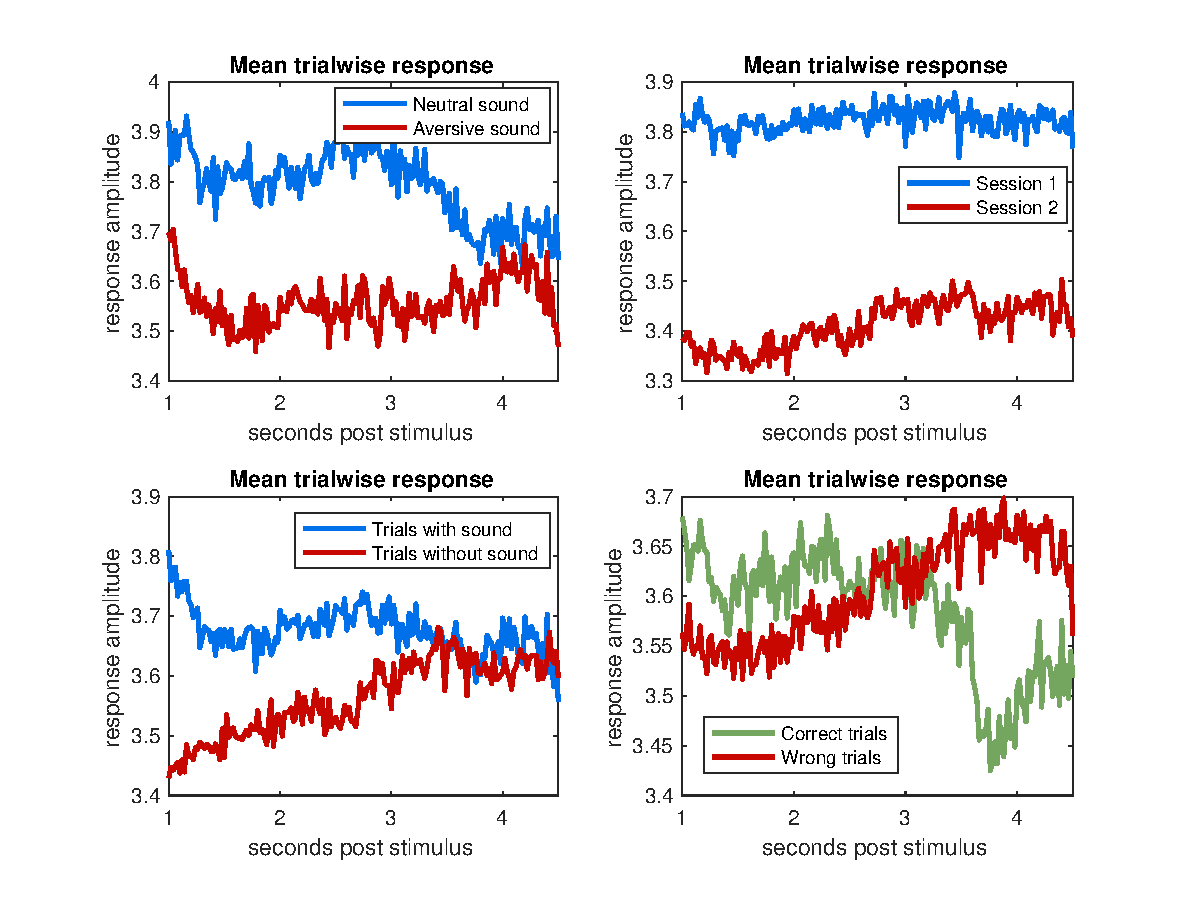
\includegraphics[width=.45\textwidth]{gsr_mean_res}
  \caption{Grand average response of SCR signal depending on several variables of interest.}
  \label{fig:gsr-mean}
\end{centering}
\end{figure}

Surprisingly, their SCR were consistently higher for the first session compared to the second. More importantly, aversive sounds do not seem to have induced a higher response in general. The crucial subplot, however, is in the bottom right. It suggests a mediocre tendency towards an elevated signal for correct trials as well as a signal drop 3.5 sec post-stimulus for trials with a prediction error. While these tendencies are far from being indisputable, they yielded the opportunity to infer \textit{canonical responses} for trials with and without prediction error, which were obtained via simple median filtering. This provided a pathway towards the first question we posed (see \hyperref[sec:intro]{introduction}). We verified to what extent inference on the beliefs is possible solely based on the physiological data obtained via the GSR device (in absence of any behavioral response). Based on the euclidean distance between the SCR of any trial with the two canonical responses, we generated a binary sequence of beliefs about the occurrence of the sound. However, examining the plain performance profiles of the inferred response traces, \autoref{fig:gsr} (left plot) reveals a significant drop for the physiologically inferred responses.
\begin{figure}[H]
\hspace{-0.7cm}
  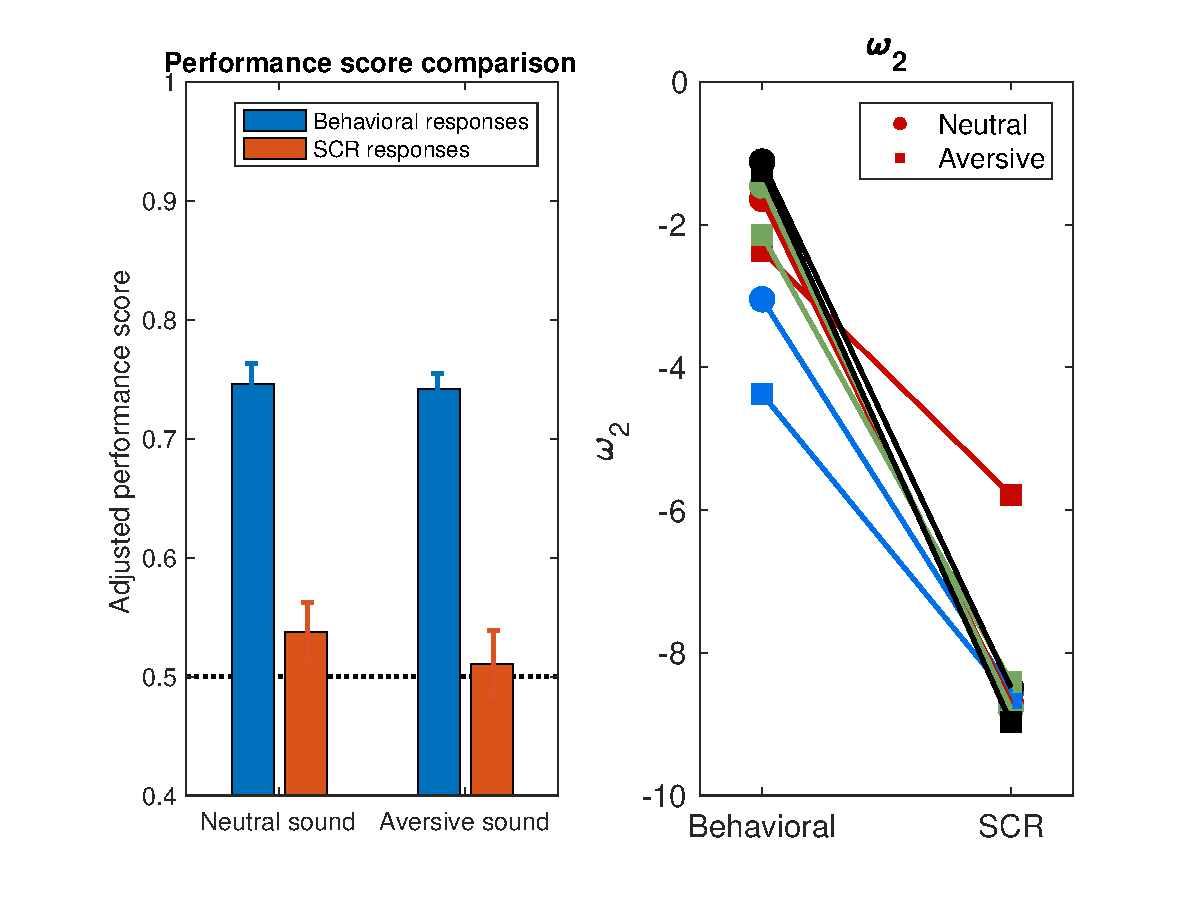
\includegraphics[width=.55\textwidth]{gsr}
  \caption{\textit{Left:} Comparing the performances of the behaviorally recorded responses with the SCR inferred beliefs. Bars indicate confidence intervals, the dotted line indicates chance level. \textit{Right:} Comparison of $\omega_2$ parameter of HGF fits for behavioral and SCR data. Behavioral does refer to the default HGF fit (Model 1).}
  \label{fig:gsr}
\end{figure}
\vspace{-5mm}
Indeed, the performance declines to a level just above chance. A binomial test could not reject the $H_0$ that the hypothetical responses derived from the SCR signal
stem from the same distribution like random responses ($p=0.11$), whereas the same test resulted in high significance ($p=1\mathrm{e}{-66}$) for the behavioral responses. 

The right plot of \autoref{fig:gsr} shows a comparison of the $\omega_2$ values of the HGF fitted to the behavioral and the SCR inferred responses. The default parameter settings were used for both models. For all participants and all sessions, a clear reduction in $\omega_2$ can be observed. As $\omega_2$ is inversely proportional to the volatility of the belief trajectory and the nature of our paradigm demands this volatility to be high in order to reach strong success rates, the drop in $\omega_2$ may be precipitated by (1) a less (hierarchical) Bayes-optimal behavior or (2) inherent inconsistencies in the SCR belief traces and consequent failure of the HGF to fit them.

Conclusively, this result does not provide evidence for our hypothesis that the beliefs about sound occurrence can be inferred from the skin conductance signal. Given that would be possible in this experiment, we had expected only marginal changes in both, the performance plot and the $\omega_2$ comparison in \autoref{fig:gsr}. In the \hyperref[sec:discuss]{discussion} we outline several reasons for why this may be the case.

The HGF fits also supply $\varepsilon_2$, a precision-weighted PE between the outcome of each auditory event and its priorly estimated probability as well as $\varepsilon_3$, a precision weighted PE  about the cue-outcome contingency. We compared the mean SCR for trials with low $\varepsilon_2$ (or $\varepsilon_3$) to the ones with high values (neglecting the error polarity). This did not unravel any significant insights.




%\subsection*{Cognitive interpretation of $\Delta\omega_2$}
%To a layman's ears, the meaning of $\omega_2$ within the HGF, i.e., \say{tonic component of the variance of the tendency}, justly appears somewhat nebulous, that is, not readily understandable in cognitive or psychological terms. This situation not only impedes a clear interpretation and communication of our experimental results, but also the translational aspirations of this variant of general modeling in a broader sense. Assuming our finding of two subgroups of different $\omega_2$-differentials, $\Delta\omega_2$ is reproducible on a more significant scale, we will now propose a cognitive perspective as a complementary interpretation to the one pertaining to the classical HGF framework. Concretely, we propose an interpretation of $\omega_2$ in terms of $\alpha$, the auxiliary parameter describing a \textsf{temporal window of integration}. \\ 
% LUKAS: bitte noch 1-2 Sätze genauere Beschreibung adden.
%Casting $\omega_2$-differences in terms of a change in the temporal window of integration naturally leads to an interpretation of our two subgroups (those with $\Delta\omega_2 > 0$ and those with $\Delta\omega_2 < 0$) in cognitive terms. Subjects whose $\omega_2$ decreased in the aversive session now seem to behave more \say{Bayes-optimally} by integrating more information from the past, and vice versa. In fact, one of our subjects has lucidly hinted at this perspective en passant, long before our theoretical considerations had matured to their current state. \\ 
%Niceüberleitung, we hypothesized that people whose temporal window of integration decreases with aversive stimuli would generally be more prone to erratic and anxious behavior in everyday life. Unfortunately however, correlating subjective measures of anxiety-proneness from our questionnaire with $\Delta\omega_2$ reveals no significant relationship.

%\begin{figure}[H]
%\centering
%\includegraphics[width=.5\textwidth]%{omega2_diff_vs_anxiety.png}%
%5\caption{$\Delta\omega_2$ versus subjective measure of anxiety-proneness.}
%\label{fig:sub2}
%\end{figure}




\section*{Discussion}
\label{sec:discuss}
In the following, we will sequentially discuss the results of the \hyperref[sec:Q]{3 questions} we raised in the introduction to motivate this project.
\\


\textbf{A. Do computational quantities also have \textit{peripheral} physiological correlates?}

Our analysis of the skin conductance response of 4 participants could not provide supporting evidence for the idea that a computational quantity like a prediction error about auditory stimulus outcome exhibits correlates encoded in peripheral physiological signals. This question was attempted by investigating to what extent inference on the belief of stimulus outcome can be made in the absence of behavioral responses. We can, however, report a difference in the SCR for correct and incorrect predictions about an auditory stimulus which may potentially be of qualitative nature. In addition, we have sketched a methodological pipeline on (1) how cognitive entities like beliefs about occurrences of sensory events may be inferred from physiological data and (2) how a quantitative comparison within established generative models of behavior can be conducted. Future projects should carefully consider amendments to the following aspects which may have caused the lack of supporting evidence:
\begin{enumerate}
\item The GSR device. Although our handcrafted setup was successfully tested prior to the experiment (it showed response increases due to physical exercising or suddenly getting scared), to our best knowledge, an \texttt{arduino} micro-controller has not been used previously in a scientific context to infer about SCR.
\item The amount of participants. Due to the \hyperref[sec:purge]{aforementioned difficulties}, our sample size ($N=4$) was insufficient to allow strong conclusions in any direction.
\item Our expectation that the SCR inferred belief traces should yield similar performance scores and $\omega_2$ distributions like the behavioral responses assumes that the behavioral responses indeed closely reflect the belief about cue-stimulus contingency (compare \autoref{fig:gsr}).
\item The "canonical" skin conductance response for the prediction error was inferred from the same trials that were used to generate the SCR belief trace. This induced an inherent bias which could have been avoided by (1) cross validation or (2) a widely accepted (actually canonical) SCR signal, similar to the hemodynamic response function in fMRI. To our best knowledge, this canonical response does not yet exist in literature, but may be a worthwhile consideration for future work in the field.
\end{enumerate}








\textbf{B. Does stimulus nature bias behavior in a sensory-motor learning task?}\\
Fitting the modified HGFs to data from neutral and aversive sessions individually and comparing the parameters revealed two subgroups in the examined cohort --- with the discriminating factor being $\omega_2$: In 4 subjects, $\omega_2$ increased, whereas in the remaining 8 subjects, it decreased. With respect to the meaningfulness of this observation, we emphatically acknowledge our awareness of the fact that drawing a dozen numbers from a normal distribution twice and subtracting them pairwise would in all likelihood yield precariously similar \say{$\Delta\omega_2$}. Only further investigations could reveal whether this observation indeed reveals itself as a red herring.\\ 
Cautionary statements aside, we further hypothesized that subjects whose $\omega_2$ increased with aversive stimuli would generally tend to behave more erratically, and vice versa. In an attempt to link $\Delta\omega_2$ to a colloquially more tangible trait, namely general anxiety-proneness, we evaluated the relationship between subjective anxiety-proneness and $\Delta\omega_2$--- unfortunately however, to little avail: the correlation of $0.37$ prohibits us from drawing strong conclusions. In short, while our results certainly hint at its existence, the degree to which aversive stimuli bias behavior has yet to be convincingly disentangled from experimental noise. \\ 
Finally, we propose a reinterpretation of $\omega_2$ in terms of a temporal window of integration, where an increase in $\omega_2$ can be understood as a decrease in the extent of the temporal window with which past information is integrated into the present belief. \\

\textbf{C. Can we derive a temporal interpretation of behavioral parameters that may serve as a  diagnostic tool in computational psychiatry?}

We developed a Pseudo-Bayesian framework to render the individual differences in $\omega_2$ and $\omega_{2}$-differentials intuitively accessible in the time domain. Specifically, we show that, under certain constraints, $\omega_{2}$ can be understood in terms of a \textsf{temporal window of integration}. This measure may prove to be useful in understanding inter-individual differences in information processing; specifically, in the dynamic integration of sensory information over time. As such, it may represent one out of the many dimensions that are essential for understanding psychiatric diagnosis. Furthermore, it is a measure that is interpretable both by researchers and clinicians inside and outside of the Bayesian community. This may allow setting up joint research projects with, e.g., experimental neuroscientists interested in the accumulation and integration of sensory evidence over time.

A Pseudo-Bayesian follow-up to this project will be addressing a set of questions and concerns: 

\begin{enumerate}
\item The similarity analysis was carried out on data that was recorded in an experiment with little to no variance of volatility. The effect of $\omega_3$ and the relation to a Pseudo-Bayesian model with non-constant $\alpha$ needs to be studied more carefully. 
\item A larger study will be carried out to compare $\omega_2$ to the $\alpha$ of the Pseudo-Bayesian fit based on the HGF trajectory and to the $\alpha$ of the Pseudo-Bayesian fit based on the binary input sequence. This will be repeated for a diverse set of behavioral responses. So far, we have primarily worked with representative samples and fits based on HGF-trajectories to define the scope and power of the models.  
\item The temporal quantities described above will be assessed in clinical and non-clinical subpopulations based on experimental recordings. 
\end{enumerate}

\section*{Acknowledgements}

First and foremost, we would like to acknowledge Prof. Klaas Enno Stephan, for passionately and eloquently planting a very valuable seed in our minds, a seed that quickly found fertile ground and grew into a strong interest and personal involvement in the field of translational neuromodeling. All TNU members and guest lecturers who gave equally insightful, entertaining and inspiring lectures or comments deserve our utmost gratitude.
Specifically, we owe our thanks to Lillian Weber, for providing invaluable, lucid feedback, disclosing some of the tricks of the trade (adjusting priors!), and assisting us in coding up the two-layer HGF configuration. Next, we acknowledge Jakob Heinzle for kindly providing the electrolyte paste that rendered our SCR measurements usable to begin with. Finally, Ethan Palmiere carefully injected some enlightening thoughts and Seraina Steiger kindly assisted us with LaTex advice. %nai bitte nöd... das sind 15 minute gsi!  



\newpage

\bibliography{TNM_bib}

\end{multicols}

\end{document}